%\documentclass[final,5p,twocolumn,10pt,number]{elsarticle}\usepackage{amsmath}\usepackage{pxfonts,amssymb}

\documentclass[review,3p,times,12pt,number]{elsarticle}\usepackage{amsmath}\usepackage{amssymb}






\usepackage{multicol,enumitem,multirow,booktabs,amsthm,subfigure}


\newlength{\smalltable}
\setlength{\smalltable}{252pt}


\newtheorem{proposition}{Proposition}
\newtheorem{definition}{Definition}


\usepackage[vlined,ruled,linesnumbered]{algorithm2e}
\SetKwComment{tcp}{/\!/\,}{}
\SetArgSty{textrm}
\SetKwProg{Procedure}{procedure}{}{end~procedure}
\SetKwProg{Function}{function}{}{end~function}
\SetKwFor{Repeat}{repeat}{times do}{end~loop}
\SetKwFunction{Move}{Move}
\SetKwFunction{Relocate}{Relocate}
\SetKwFunction{EvalMove}{EvalMove}
\SetKwFunction{Valid}{ValidTasks}
\SetKwFunction{Largest}{LargestPriorityTasks}
\SetKwFunction{EvalTask}{EvalTask}
\SetKwFunction{MoveNeed}{MoveNeed}
\SetKwFunction{Fill}{Fill}
\SetKwFunction{BiReceiver}{BiReceiver}
\SetKwFunction{BiSender}{BiSender}
\SetKwFunction{Interim}{Interim}
\SetKwFunction{InterimFull}{InterimFull}
\SetKw{Break}{break~while}

\renewcommand{\citet}[1]{\citeauthor{#1}~\citep{#1}}
\makeatletter
\def\NAT@def@citea{\def\@citea{\NAT@separator}}
\makeatother


\usepackage[colorlinks=true]{hyperref}
%\AtBeginDocument
{
\hypersetup{linkcolor =magenta,
anchorcolor =red,
citecolor =cyan,
filecolor =red,
menucolor =red,
runcolor =red,
urlcolor =cyan
}
}


\usepackage{caption}
\captionsetup[figure]{font=small}
\captionsetup[table]{skip=0.5ex,font=small}



\renewcommand{\gets}{\coloneqq}
\renewcommand{\emph}[1]{\textbf{\textit{#1}}}



\newcommand{\mss}{s^\mathrm{src}}
\newcommand{\mds}{s^\mathrm{dst}}
\newcommand{\mts}{s^\mathrm{tmp}}




\newcommand{\setalgo}{\linespread{1}\fontsize{10}{12}\selectfont}
\newcommand{\settab}{\linespread{1}\fontsize{10}{12}\selectfont}

\sloppy


\begin{document}

\begin{frontmatter}

\journal{EJOR}
\title{A feasibility-based heuristic for the container pre-marshalling problem}
\author[cityu]{Bo Jin}
\ead{msjinbo@cityu.edu.hk}
\author[cityu]{Andrew Lim\fnref{lim}}
\ead{alim.china@gmail.com}

\author[shu]{Ning Wang\corref{cor}}
\ead{ningwang@shu.edu.cn}

\author[syu]{Zizhen Zhang}
\ead{zhangzizhen@gmail.com}

\cortext[cor]{Corresponding author. Tel: +86 18930400865}



\address[cityu]{Department of Management Sciences, City University of Hong Kong, Tat Chee Avenue, Kowloon Tong, Hong Kong}
%\address[andrew]{School of Physical and Mathematical Sciences, Nanyang Technological University, Singapore 637371, Singapore}
\fntext[lim]{Andrew Lim is currently on no pay leave from City University of Hong Kong.}
\address[shu]{Department of Information Management, School of Management, Shanghai University, Shanghai, China}
\address[syu]{School of Mobile Information Engineering, Sun Yat-Sen University}

\begin{abstract}

This paper addresses the container pre-marshalling problem (CPMP) which rearranges containers inside a storage bay to a desired layout.
By far, target-driven algorithms have relatively good performance among all algorithms; they have two key components: 1) containers are rearranged to their desired slots one by one in a certain order; and 2) rearranging one container is completed by a sequence of movements. Our algorithm improves the performance from the aforementioned two components.
Instead of rearranging containers in the descending order of their group labels (traditional idea), this paper determines the order as the algorithm goes on by an evaluation function. To efficiently explore the enlarged search space, we are the first one to come up with a concept of state feasibility to cut branches.
%State feasibility can recognize a useless branch without really carrying out a sequence of movements to reach that branch.
In addition, we improve the sequence of movements by techniques such as pre-extreme avoidance and tier protection.
Computational experiments showcase that the performance of our proposed heuristic is better than other heuristics.
\end{abstract}

\begin{keyword}
container pre-marshalling problem \sep feasibility-based heuristic
\end{keyword}
\end{frontmatter}




\section{Introduction}



Since the commencement of containerization, the global use of standardized containers has dramatically improved international trade. Containers enable the smooth flow of goods between multiple transportation modes without directly handling the freight. Over the years, stringent requirements such as just-in-time operations from consignors have created additional challenges for the container transportation industry.

Container yards --- the spaces dedicated to the transshipment, handover, loading, consolidation, maintenance, and storage of containers --- are key components of maritime container terminals. Some yards act as exchange venues for container transfers between different transportation modes while others are used as caches for temporary storage or as warehouses for long-term storage.

Generally speaking, a container yard is divided into several yard blocks, each of which consists of several parallel bays.  A bay is formed by a row of stacks. Usually the containers stored in the same bay have the same dimensions. Equipments such as rubber tyre gantry cranes, rail-mounted gantry cranes, and reach stackers are frequently used in container yards. Figure~\ref{fig:block} illustrates an example of a yard block.

\begin{figure}[htbp]
\centering
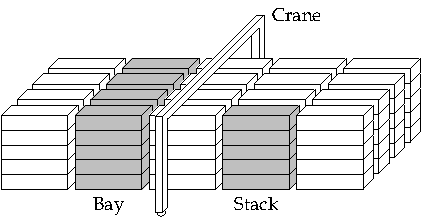
\includegraphics{figs/block.pdf}
\caption{Yard block.}
\label{fig:block}
\end{figure}

Containers in the same stack are organized in a last-in-first-out matter. To retrieve containers placed in lower levels, containers on top of them must be relocated to other places (other slots or the yard) first. Such forced movements are known as container reshuffles.
Container pre-marshalling problem (CPMP) addresses the reorganization of containers inside a storage area such that no reshuffling is further required when containers are retrieved. Hence, CPMP is to improve terminals' performance level, including their throughput rate per berth and the turnaround time of vessels or road trucks~\citep{kim2015}.

The CPMP can be formally defined as follows: containers are initially placed in several stacks. These stacks form a bay. Each container is marked with a group label. CPMP is to rearrange the containers within the bay, so that containers in each stack are placed in a descending order of group labels from bottom to top. The objective is to carry out the rearrangement with the fewest number of container movements.
This paper investigates the CPMP, and it is assumed that the retrieval order of the containers is known beforehand and no container arrives at or leaves from the bay during pre-marshalling.

This paper makes two main contributions to the literature.
%First, a feasibility-based heuristic is proposed. The proposed heuristic is a target-driven algorithm, therefore it can be implemented solely or be combined with existing frameworks in the literature such as tree search, greedy or GRASP.
One contribution is the idea behind the proposed heuristic. In the traditional algorithms, containers are allocated according to a certain order, such as the descending order of their groups \citep{exp2012}; in this research, the order to allocate containers is not fixed beforehand, but rather that it is decided as the algorithm goes on. This innovation undoubtedly enlarges the search space and decreases the search efficiency. To avoid efficiency decrease, we propose the concept of state feasibility to check the feasibility of allocating a certain container before we actually allocate it. The time complexity of check feasibility is only $\mathcal O(G)$, here $G$ is the number of groups. Our paper is the first work that uses feasibility to cut branches in CPMP algorithms.
Another contribution is that the proposed heuristic performs outstandingly on both dense and loose instances, compared with existing heuristics. The better performance is thanks to the techniques used, such as state stability, dead-end states avoidance and tier-protection indicator which will be explained in Section~\ref{sec:fbh}.

The remainder of this paper is structured as follows. Section~\ref{sec:literature} reviews existing approaches in the literature. Section~\ref{sec:problem} gives a mathematical description of the problem and lists the notation used throughout this paper. The concept of state, state feasibility and stable state are introduced in Section~\ref{sec:state}
Comprehensive description of the heuristic and associate techniques are explained in Sections~\ref{sec:fbh}. Section~\ref{sec:experiment} illustrates the results of our computational experiments, and the last section concludes this paper and identifies future research directions.

\section{Recent work}
\label{sec:literature}
According to recent reviews~\citep{carlo2014,lehnfeld2014}, problems related to or caused by container reshuffles at terminals include three major kinds of decision problems. The first problem is the container relocation problem~\citep{jin2015} which minimizes the total operational cost in the container retrieval process. The operational cost is commonly measured by the number of relocations conducted or the total operational time. The second is the container pre-marshalling problem addressed in this paper. The third problem is container stacking problem which decides the selection of storage locations or sequences the movements of cranes for arriving containers~\citep{Dayama2014}.


To the best of our knowledge, only seven works study the solutions to the pre-marshalling problem, which is rather few compared with other problems in ports, such as berth allocation problems and quay crane scheduling problems. The aforementioned two problems have been studied in more than 120 publications just since 2009 \citep{Bierwirth2015}. One reason behind is that the variants of pre-marshalling problem by far are few. Known variants appear in \citet{wang2015} which considers truck lanes and in \citet{Huang2012} which requires containers of different groups be separately located in the final layout. In the following, the only seven works will be discussed in sequence.

\citet{lee2007} develop an integer programming model for the CPMP\@. In this work, the problem is formulated as a multi-commodity network flow problem. The overall network is divided into several subnetworks, with each subnetwork representing an intermediate layout. The nodes in a subnetwork correspond to the slots that accommodate containers, and the commodities correspond to the containers stored in the bay. Every valid flow in the network represents a solution to the pre-marshalling problem. The model provides an innovative viewpoint to the problem; however, its performance is limited because the network is too large even for a small instance.


\citet{cas2009} provide a greedy heuristic, the corridor method, for solving the problem. The heuristic selects the direction of movements in a randomized manner according to the attractiveness of available successors confined by the corridor. The attractiveness is measured by an estimated number of additional relocations needed for the particular successor.
A local improvement procedure is also conducted to accelerate the heuristic process.

A neighborhood search is proposed by \citet{lee2009}, which repeatedly modifies the current solution until some termination condition is met. Unlike other existing solution-construction approaches, the neighborhood search is required to start from a pre-generated initial solution.
A feasible solution can be further improved by a four-step procedure, and the diversity of the neighborhood is raised by multiple subroutines. The main drawback of the approach is the unreliability of random solution modifications, i.e., the feasibility of the resultant new solutions are not always ensured.

\citet{bort2012} describe a tree search procedure for solving the problem.
In the tree search structure, solutions are constructed by compound moves instead of single moves. Moves are classified into four types, and only the most promising ones are adopted in the branching scheme.

There are two studies in the literature regarding heuristic approaches. They adopt the same heuristic strategy that containers are handled in reverse of their retrieval order.

\citet{exp2012} provide the first group-oriented heuristic for the CPMP. Their method iteratively handles containers in a descending order of container group values. After handling all containers with a specific group value, a stack filling process is applied to reduce the number of disorderly containers in the bay.

\citet{Huang2012} solved two variants of CPMP by a heuristic algorithm. One variant is commonly seen which allows containers of different groups to mix within a bay. The other variant is newly proposed, which requires containers of different groups be separately located in the final layout.

\citet{wang2015} propose a target-guided heuristic (TGH) and two beam search algorithms. The TGH also handles containers in a descending order of the container group values. The method to determine container handle order and the way to handle a container are improved.
This work can solve instances of different densities well, especially dense instances with fewer empty slots.

\section{Problem description and notations}
\label{sec:problem}

The CPMP is restricted to the bay size, or more precisely, the dimensions of the operating cranes. As shown in Figure \ref{fig:bay}, an instance (problem input) includes an initial layout of $N$ containers, which are distributed in a single bay with $S$ stacks ($S\ge 3$) and $H$ tiers ($H\ge 2$) with $E$ empty slots ($E=SH-N$, $E\ge 2$) left.

\begin{figure}[htbp]
\centering
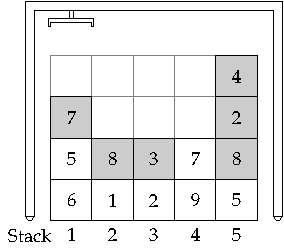
\includegraphics{figs/bay.pdf}
\caption{A container bay.}
\label{fig:bay}
\end{figure}

Each container is labeled with a group value $g \in[1,G]$. A container is \emph{orderly} if it is supported directly by the ground or another orderly container with equal or larger group value; otherwise, it is \emph{disorderly}. Other phrases which have the same meaning of ``orderly{\slash}disorderly'' in recent literature include ``well{\slash}badly placed''~\citep{bort2012}, ``well-{\slash}non-located''~\citep{exp2012}, and ``clean{\slash}dirty''~\citep{wang2015}.

Figure~\ref{fig:bay} gives an example of a bay for which $S=5$, $H=4$, and $N=13$. Containers are represented by boxes with their group values marked inside. In addition, boxes with gray background are disorderly containers.
The objective of the CPMP is to find an optimized sequence with the fewest container movements, by which all containers are rearranged to be orderly.
The movement sequence is called ``applied to" the CPMP case.



%\section{Notation}
%\label{sec:notation}
%
%\newlength{\mylongest}
%\settowidth{\mylongest}{$\alpha(s^+,s)$}
%\addtolength{\mylongest}{\labelsep}
%\SetLabelAlign{LabelCenter}{\makebox[\mylongest]{#1}}

To better describe the solution to CPMP, we represent layout-related items mathematically.
The tier and stack numbers of the bay are labeled from bottom to up and left to right, respectively.
Let $\mathbb{S}=\{1,\dots,S\}$ be the set of stacks. Hereafter, for simplification of description, when a stack $s$ is mentioned without declaring its domain, it is assumed that $s\in\mathbb{S}$. The height of stack $s$ is denoted by $h(s)$ and $e(s)=H-h(s)$ denotes the number of empty slots in $s$. Note that the height of stacks should not exceed $H$.
The orderly height (number of orderly containers) of $s$ is denoted by $o(s)$.

The slot positioned at $t$-th tier of stack $s$ is denoted by $(s,t)$.
The group value of a container $c$ is denoted by $g(c)$.
Likewise, the group value of a container located in slot $(s,t)$ is denoted by $g(s,t)$.






%Let us define the capability of an occupied slot $(s,t)$ by $q(s,t)=p(s,t)$ if the container inside is orderly, otherwise $q(s,t)=0$; specifically, regarding the ground as an occupied slot at tier $0$ with priority value $P$. Thus, we can easily verify the placement of a container $(s,t)$ by checking whether $p(s,t)\le q(s,t-1)$.

%The notation for describing the problem is as follows.
%
%\subsubsection*{I\@. Global constants}
%
%\begin{enumerate}[noitemsep, align=LabelCenter,labelwidth=\mylongest,leftmargin=!]
%\item[$N$] number of containers
%\item[$S$] number of stacks
%\item[$H$] height limitation of stacks
%\item[$G$] number of groups
%\item[$E$] number of empty slots, $E=SH-N$
%\item[$U$] number of unreachable tiers, $U=\max\{H-E,0\}$
%\item[$\mathbb{C}$] set of containers
%\item[$\mathbb{S}$] set of stacks, $\mathbb{S}=\{1,\dots,S\}$
%\end{enumerate}
%
%
%
%\subsubsection*{II\@. Common symbols and functions}
%\begin{enumerate}[noitemsep, align=LabelCenter,labelwidth=\mylongest,leftmargin=!]
%\item[$\mathsf{L}$] layout
%\item[$c$] container
%\item[$s$] stack index
%\item[$t$] tier index
%\item[$g$] group value
%\item[$(s, t)$] slot or the container located in
%\item[$h(s)$] height of stack $s$, vectorized as $\boldsymbol{h}$
%\item[$e(s)$] number of empty slots in stack $s$, $e(s)=H-h(s)$
%\item[$o(s)$] orderly height of stack $s$, vectorized as $\boldsymbol{o}$
%\item[$f(s)$] fixed height of stack $s$, vectorized as $\boldsymbol{f}$
%\item[$(\mathsf{L},\boldsymbol{f})$] state
%\item[$g(c)$] group value of container $c$
%\item[$g(s,t)$] group value of container $(s,t)$
%%\item[$q(s,t)$] capability of an occupied slot $(s,t)$
%%\item[$q^f(s)$] capability of the top fixed slot in stack $s$, $q^f(s)=q(s,f(s))$
%\end{enumerate}
%
%\subsubsection*{III\@. Resource-{\slash}demand-related functions}
%\begin{enumerate}[noitemsep, align=LabelCenter,labelwidth=\mylongest,leftmargin=!]
%\item[$d(p)$] order-$p$ demand, i.e., the number of unfixed containers with priority $p$
%\item[$D(p)$] order-$p$ accumulate demand, $D(p)=\sum_{\varphi=p}^P d(\varphi)$, vectorized as $\boldsymbol{D}$
%\item[$r(p)$] order-$p$ resource, $r(p)=\sum_{q^f(s)=p} (H-f(s))$
%\item[$R(p)$] order-$p$ accumulate resource, $R(p)=\sum_{\varphi=p}^P r(\varphi)$, vectorized as $\boldsymbol{R}$
%\item[$\Delta(p)$] order-$p$ surplus, $\Delta(p)=R(p)-D(p)$, vectorized as $\boldsymbol{\Delta}$
%\end{enumerate}
%
%The following is the extra notation used to describe the proposed algorithms.
%
%
%\subsubsection*{IV\@. Task-related symbols}
%\begin{enumerate}[noitemsep, align=LabelCenter,labelwidth=\mylongest,leftmargin=!]
%\item[$c^*$] target container
%\item[$s^+$] stack of the target container
%\item[$t^+$] tier of the target container
%\item[$s^-$] aim stack
%\item[$b$] number of blocking containers
%\item[$a$] number of slots available for blocking containers
%\end{enumerate}
%
%\subsubsection*{V\@. Extra symbols}
%\begin{enumerate}[noitemsep, align=LabelCenter,labelwidth=\mylongest,leftmargin=!]
%\item[$\mss$] source stack (sender) of a move
%\item[$\mds$] destination stack (receiver) of a move
%\item[$\mts$] interim stack for temporarily storing the target container
%\item[$\vec{v}$] evaluation tuple of a move, lexicographically comparable\item[$\mathbb{R}$] receiver set
%\item[$\mathbb{I}$] set of potential interim stacks
%\item[$\mathbb{F}$] set of potential interim stacks which are  currently full
%\item[$\mathbb{T}$] set of valid tasks
%\end{enumerate}
%
%\subsubsection*{VI\@. Extra functions}
%\begin{enumerate}[noitemsep, align=LabelCenter,labelwidth=\mylongest,leftmargin=!]
%\item[$g(s)$] stable height of stack $s$, vectorized as $\boldsymbol{ g}$
%\item[$m(s)$] messiness (largest unstable priority value) of stack $s$, $m(s)=\max_{ g(s)<t\le h(s)}p(s,t)$
%\item[$\alpha(s^+,s)$] number of slots available after the move from stack $s^+$ to stack $s$
%\item[$\delta(p,q)$] demand between $p$ exclusive and $q$ inclusive, $\delta(p,q)=\sum_{\varphi=p+1}^{q}d(\varphi)$
%\end{enumerate}


\section{State and State Feasibility}
\label{sec:state}
\begin{definition}[Fixed containers]
A fixed container is an orderly container and not allowed to be moved in the following movement sequence.
\end{definition}
If a container is a fixed container, then the containers under it must be fixed containers.
\begin{definition}[State]
A state $(\mathsf{L},\boldsymbol{f})$ is a pair composed of a layout $\mathsf{L}$ and a fix vector $\boldsymbol{f}$.
\end{definition}
The {fix} vector $\boldsymbol{f}$ indicates the number of fixed containers (fixed height) in each stack of $\mathsf{L}$. $\boldsymbol f(s)$ is the $s$th element. Fixed and unfixed containers are separated by a line (a skyline), as shown in Figure~\ref{fig:skyline}.
In Figure \ref{fig:exp1}, $\boldsymbol f=(2,3,1)$; in Figure \ref{fig:exp2}, $\boldsymbol f=(2,3,0)$.

\begin{figure}[htbp]
\centering
\subfigure[]{
    \label{fig:exp1}
    \resizebox{0.35\textwidth}{!}{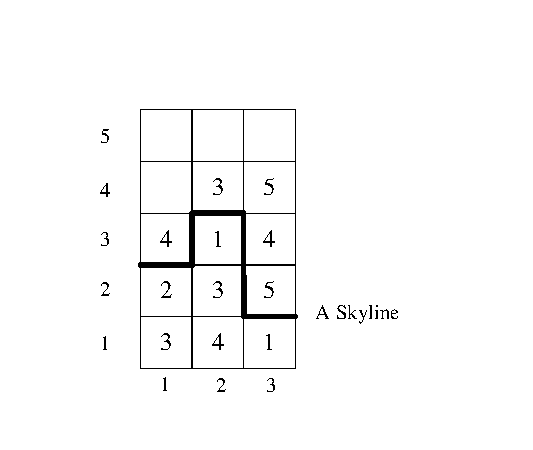
\includegraphics{figs/exp1.pdf}}}
\subfigure[]{
    \label{fig:exp2}
    \resizebox{0.35\textwidth}{!}{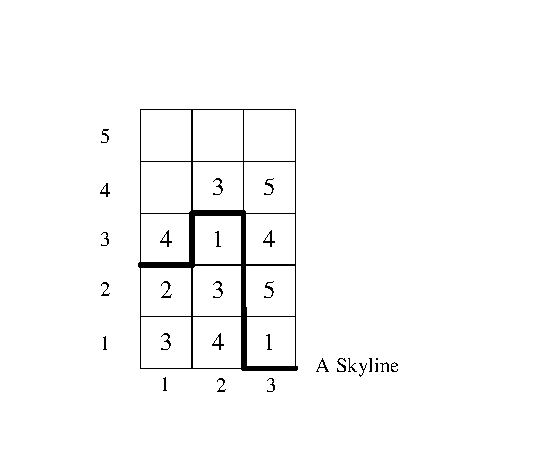
\includegraphics{figs/exp2.pdf}}}
\caption{Fix vector and skyline}
\label{fig:skyline}
\end{figure}


It is noteworthy that if two states have the same layout but different fix vectors, then they are two different states, just like Figure~\ref{fig:exp1} and~\ref{fig:exp2}.

\begin{definition}[Feasibility of a state]
A state $(\mathsf{L},\boldsymbol{f})$ is feasible if there exists a movement sequence that can convert $\mathsf{L}$ to an orderly layout without moving fixed containers indicated by $f$.
\end{definition}

The necessary condition for state feasibility has been talked about in \citet{wang2014}. To make the content self-contained, we briefly explain it in this paper. Containers above the skyline can be moved, therefore slots and containers above the skyline now are separately considered. In one stack $s$, suppose the smallest group label under the skyline is $g$, then $H-f(s)$ slots above the skyline can only be placed with containers with group label no larger than $g$, or the stack is disorderly. In such a situation, we say stack $s$ has $H-f(s)$ slots with group label $g$. If the skyline of stack $s$ is the ground , then $s$ has $H$ slots with group label $G$.
For example, in Figure \ref{fig:exp2}, stack 1, 2, 3 have 3, 2, 5 slots with group label 2, 1, 5, respectively. The total number of slots with group label $g$ in the whole bay is denoted as $r(g)$ (resource of group $g$). Similarly, the number of unfixed containers with group label $g$ is denoted as $d(g)$ (demand of group $g$).
For a feasible state, the slots available for group $g$ must be more than the demand of group $g$. That is,
\begin{equation*}
\sum^G_{i=g+1}r(g)-\sum^G_{i=g+1}d(g)+r(g)\ge d(g)
\end{equation*}
which is equivalent to
\begin{equation*}
\sum^G_{i=g}r(g)\ge \sum^G_{i=g} d(g)
\end{equation*}

Denote $R(g)=\sum^G_{i=g}r(g)$ and $D(g)=\sum^G_{i=g}d(g)$. $\boldsymbol R$ and $\boldsymbol D$ are the two G-dimension vectors with elements $R(g)$ and $D(g)$, respectively. The above condition is expressed as $\boldsymbol{\Delta}=\boldsymbol{R}-\boldsymbol{D}\ge \boldsymbol{0}$. Here $\boldsymbol \Delta$ is called `surplus vector'.

\begin{proposition}[Necessary condition for state feasibility]\label{prop:necessary}
A necessary condition for a feasible state $(\mathsf{L},\boldsymbol{f})$ is $\boldsymbol{\Delta}=\boldsymbol{R}-\boldsymbol{D}\ge \boldsymbol{0}$.
\end{proposition}



Take the layouts in Figure~\ref{fig:exp1} and \ref{fig:exp2} as an example, and Table~\ref{tab:feasible} shows the surplus vectors for both cases. Case a is infeasible as only $\Delta(1)\ge0$; while the feasibility of Case b is not sure since the above conditions are necessary conditions. Intuitively, it can be seen that none of the three stacks in Figure~\ref{fig:exp1} can accommodate containers with group label 5 orderly, and this is the reason why Case a is infeasible.

\begin{table}[htbp]
\caption{Computation for the surplus vector.}
\centering

\begin{tabular}{c|c|c|c|c|c||c|c|c|c|c|c}
\hline
\multicolumn{6}{c||}{Case a} & \multicolumn{6}{c}{Case b}\\
\hline
$g$ & $d(g)$ & $D(g)$ & $r(g)$ & $R(g)$ & $\Delta(g)$ & $g$ & $d(g)$ & $D(g)$ & $r(g)$ & $R(g)$ & $\Delta(g)$\\
\hline
1   & 0      & 5      & 6      & 9      & 3           & 1   &  1     & 6       & 2      & 10     & 4\\
2   & 0      & 5      & 3      & 3      & -2          & 2   &  0     & 5       & 3      & 8      &  3\\
3   & 1      & 5      & 0      & 0      & -5          & 3   &  1     & 5       & 0      & 5      &  0\\
4   & 2      & 4      & 0      & 0      & -4          & 4   &  2     & 4       & 0      & 5      &  1\\
5   & 2      & 2      & 0      & 0      & -2          & 5   &  2     & 2       & 5      & 5      &  3\\
\hline
\end{tabular}
\label{tab:feasible}
\end{table}

It is noteworthy that if only one container $c$ is unfixed in a state $(\mathsf{L},\boldsymbol{f})$, and the surplus vector $\boldsymbol{\Delta}\ge 0$, then at most one movement is need to convert the layout to a feasible layout. As $\boldsymbol{\Delta}\ge 0$, and $D[g(c)]=d[g(c)]=1$, we have $S[g(c)]>1$, i.e., there is at least one slot which can accommodate $c$ orderly. We just need $c$ to the slot.


\begin{definition}[Container stability]
Given a feasible state, a disorderly container is unstable. For any orderly container $c$ in slot $(s,t)$, try to fix container $c$ and those underneath it; if the resultant state remains feasible, $c$ is stable. Otherwise, $c$ is unstable.
\end{definition}

According to the definition, an unstable container cannot be fixed in the current slot even if it is orderly, because the resultant state will be infeasible. Unstable must to be moved in the future. Denote the stable height (number of stable containers) of stack $s$ by $ sh(s)$, then we have $\boldsymbol{f}\le \boldsymbol{sh}\le \boldsymbol{o}\le \boldsymbol{h}$. If a container $c$ is stable in stack $s$, we say stack $s$ \emph{stabilizes} container $c$.

Figure~\ref{fig:stable} gives an example of a state. Fixed containers are labeled with a solid square. Unstable containers are highlighted with gray background. Notice that the container $(2,1)$ with group value $6$ is orderly but unstable.

\begin{figure}[htbp]
\centering
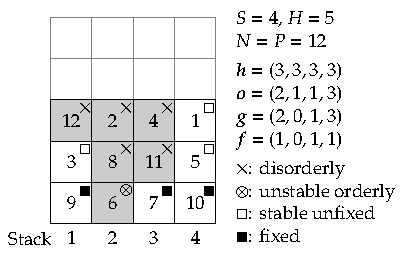
\includegraphics{figs/stable.pdf}
\caption{Stability of containers.}
\label{fig:stable}
\end{figure}

An orderly but unstable container indicates that its orderliness is valueless because it definitely requires at least one reshuffle.
Using the concept of container stability instead of container orderliness is more precise.
For example, when selecting the placement of a blocking container, if the container is orderly but unstable after moving to a stack, then the attractiveness of such a movement should be reconsidered.

Note that the stability of containers should be recomputed after any container is fixed.

\begin{definition}[Extreme state]
A state $(\mathsf{L},\boldsymbol{f})$ is called an extreme state if $|\{s\in\mathbb{S}: f(s)=H\}|= S-2$.
\end{definition}

The definition of extreme state is to emphasize the especial case where $S-2$ stacks are fully fixed. In such a case, unfixed containers can only be moved between two stacks, say $a$ and $b$; the case is feasible if and only if one of the following conditions is satisfied:
\begin{enumerate}
\item Both stacks $a$ and $b$ are orderly;
\item Stack $a$ is orderly, and stack $b$ is disorderly. Disorderly containers in $b$ can be allocated to $a$ and $a$ is still orderly after the allocation.
\end{enumerate}

\begin{definition}[Dead-end state]
A state is called a dead-end state if it is an infeasible extreme state.
\end{definition}

The dead-end states are infeasible, therefore we should avoid generating them.
We have the following proposition:

\begin{proposition}[Existence of dead-end states]\label{prop:tricky}
No dead-end state can be generated whatever movements and fixed vectors are applied to cases with $E\ge2(H-1)$. For cases with $E<2(H-1)$, there exist possibilities that the algorithm falls into a dead-end state.
\end{proposition}
When $E\ge2(H-1)$, it has $N\le SH-2H+2$, even though all containers are fixed, there are at most $S-2$ stacks fully occupied with fixed containers: 1) if there are fewer than S-2 stacks fully occupied, the state is not a dead-end state; 2) if there are S-2 stacks fully occupied, there are at most two extra containers in the left two stacks. The state is not a dead-end state, either. For cases with $E<2(H-1)$, there exist possibilities that the algorithm falls into a dead-end state.
As shown in Figure \ref{fig:non-dead-end}, it has $E\ge2(H-1)$, and it has no chance to generate dead-end states. In Figure~\ref{fig:dead-end} with $E<2(H-1)$, when $\boldsymbol f=(0,0,5,5)$, the state is a dead-end state.
\begin{figure}[htbp]
\centering
\subfigure[]{
    \label{fig:non-dead-end}
    \resizebox{0.2\textwidth}{!}{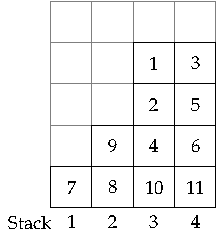
\includegraphics{figs/non-dead-end.pdf}}}
\subfigure[]{
    \label{fig:dead-end}
    \resizebox{0.2\textwidth}{!}{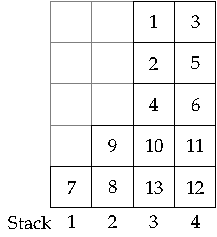
\includegraphics{figs/dead-end.pdf}}}
\caption{Existence of dead-end states}
%\label{fig:skyline}
\end{figure}

\section{Feasibility-based heuristic}
\label{sec:fbh}

In this section, a feasibility-based heuristic (FBH) is developed for solving the CPMP\@. The proposed heuristic is a target-driven algorithm. Target-driven algorithms have appeared in other works\citep{exp2012,wang2015}: generally, containers (targets) are rearranged to certain slots one by one, and each rearrangement is achieved by a sequence of movements. The heuristic can be implemented solely, then it is a greedy algorithm; the heuristic can also be the major component of other frameworks, such as GRASP and beam search.
Target-driven algorithms are effective among all existing algorithms, and our algorithm in this work is more effective. We optimize the order of rearranging containers as well as the sequence of movements in one rearrangement.

The optimization is due to the concept of state feasibility. This is why our algorithm is called feasibility-based heuristic.
Before really rearranging a certain container, the feasibility of rearrangement is checked. If the rearrangement is infeasible, then we give up this rearrangement.
Due to the feasibility, we can explore larger space without sacrificing efficiency: the order to rearrange containers is not fixed beforehand, but rather that it is decided as the algorithm goes on.






\subsection{Heuristic framework}
According to \citet{wang2014}, in dense instances such that $E<H$, for a stack $s$, only the top $\sum_{i\neq s}e(i)$ containers can be moved to other stacks. The immovable number of containers (unreachable tiers) for any stack is $U=H-\sum_ie(i)=H-E$.
Containers in the bottom $H-E$ tiers of the bay are unreachable, that is, no sequence can move these containers.
In loose instances such that $E\ge H$, all containers in a stack are movable.
Let $U=\max\{H-E,0\}$ denotes the number of unreachable tiers for any instances.

%Containers above tier $U$ are reachable containers; reachable containers can be permuted into any wanted arrangement.
The feasibility-based heuristic first constructs the initial state according to the unreachable tiers. In the initial state, $\mathsf L$ is the initial layout $\mathsf{L}^0$ and containers in unreachable tiers are fixed, i.e., $\boldsymbol f=U\cdot\boldsymbol{1}$, where $\boldsymbol 1$ is a S-dimension all-ones vector.

Starting from the initial state, the heuristic repeatedly fixes a target container $c^*$ to a target stack $s^*$. Stack $s^*$ has $f(s^*)$ fixed containers; hence, $c^*$ is fixed at tier $f(s^*)+1$. The algorithm continues until all containers are fixed. The procedure of the heuristic is concisely described in Algorithm~\ref{algo:fbhs}.

\begin{algorithm}[htbp]
\caption{Feasibility-based heuristic.}
\label{algo:fbhs}


\setalgo


\Begin
{
  $(\mathsf{L},\boldsymbol{f})\gets (\mathsf{L}^0,U\cdot\boldsymbol{1})$\;
  \Repeat{$N-SU$}
  {
    $(c^*\rightarrow s^*)\gets\textrm{the chosen valid task}$\;
    $\mathsf{L}$ = resultant layout after moving $c^*$ to $s^*$\;
    $f(s^*)\gets f(s^*)+1$\;
  }
}

\end{algorithm}

The procedure of choosing a target container $c^*$ and a target stack $s^*$ and the procedure of moving $c^*$ to $s^*$ will be explained in the following section.

The advantage of fixing containers one by one lies in twofold: 1) movements are more target-oriented. Some works such as ~\cite{bort2012} move a container each time, but they don't have a clear aim. Hence, it is difficult to measure the benefit of moves and moreover, moves are blind: a container can be unnecessarily moved from stack $a$ to $b$ in a round and then moved from stack $b$ to $a$ after several rounds. 2) fixed containers are not allowed to be moved. But unfixed orderly containers are allowed to be moved. This can distinguish fixed and unfixed orderly containers. Even though both are orderly, the statuses of both kinds of containers are totally different. In works which does not distinguish fixed and unfixed containers, some containers which do not need moved (fixed containers in our context) are involved in the movements.


\subsection{Valid task}
\label{sec:valid}

At every step of the heuristic, a {task} determines an unfixed container (target container) and a destination stack (target stack). A container--stack pair $c\rightarrow s$ is a valid task for the current state $( \mathsf{L},\boldsymbol{f})$ only if
\begin{itemize}
\item $c$ is unfixed,
\item $f(s)<H$,
\item $g(c)\le g(s,f(s))$, and
\item $\Delta(\varphi)\ge H-f(s), \varphi \in (g(c),g(s,f(s))]$.
\end{itemize}

The first condition is easy to understand. The second condition ensures that $s$ has a slot to accommodate $c$. The third condition makes sure that the group label of $c$ is no larger than that of the highest fixed container of $s$, here, $g(c)$ and $g(s,f(s))$ denotes the group labels of $c$ and highest fixed container of $s$, respectively.
The last condition ensures the non-negativity of the resultant surplus vector. If $c$ is moved to $s$, then the $g(c)$th element of demand vector $d[g(c)]$ decreases 1, i.e., $d'[g(c)]=d[g(c)]-1$, while other elements do not change. In the meanwhile, for the resource vector, $r'[g(s,f(s))]=r[g(s,f(s))]-(H-f(s))$ while $r'[g(c)]=r[g(c)]+H-f(s)-1$, and other elements do not change. Then for $\varphi \in(g(c),g(s,f(s))]$, the feasible condition in the new layout is $D'(\varphi)=\sum_{g\ge \varphi}d'(g)=D(\varphi)\le R'(\varphi)=\sum_{g\ge\varphi}r'(g)=R(\varphi)-(H-f(s))$, i.e., $\Delta(\varphi)\ge H-f(s)$.

Pairs satisfy the above conditions compose a set $\mathbb T$. However, the above conditions are only necessary conditions, so the feasibility of the resultant state is not sufficiently ensured, due to the possibility of dead-end states.

There are three methods for resolving the dead-end state issue.
\begin{enumerate}
\item Prevent from entering an extreme state when deciding the next task;
\item Design an ideal task accomplishment procedure that makes the resultant extreme state feasible;
\item Allow entering a dead-end state and relabel a fixed container as unfixed to run away from the dead-end state.
\end{enumerate}

Our previous work~\citep{wang2015} adopts the last method listed above. When the algorithm enters into a dead-end state, the algorithm relabels a fixed container as unfixed and moves it to a temporary slot; then the state becomes non-dead-end. After taking a sequence of movements, the relabeled container is recovered to its original slot. The disadvantage of such a choice is that running away from existing dead-end states costs many movements and these movements are unnecessary per se. A more choice is to avoid resulting in dead-end states when choosing valid tasks.

\begin{definition}[Pre-extreme state]\label{def:pre-tricky}
A feasible state is a pre-extreme state if $|\{s\in\mathbb{S}: f(s)=H\}|=S-3$, $|\{s\in\mathbb{S}: f(s)=H-1\}|\ge 1$ and $\sum_{s\in\mathbb{S}}f(s)<N-2$.
\end{definition}
The algorithm only explores state $(\mathsf{L},\boldsymbol{f})$ which satisfy the necessary condition for state feasibility (see Proposition \ref{prop:necessary}).
When only three stacks have available slots while the other $S-3$ stacks are fully fixed ($|s \in \mathbb S : f(s)= H| = S- 3$), and at least one stack has only one available slot left $|s \in \mathbb S : f(s) = H-1| \ge 1$, let us investigate the validity of performing a task $c\rightarrow s$ with $f(s)=H-1$ based on the number of remaining unfixed containers.

1. If $\sum_{s\in\mathbb{S}} f(s) = N$, all the containers are fixed, the algorithm terminates with an orderly layout.

2. If $\sum_{s\in\mathbb{S}} f(s) = N-1$, only one container remains unfixed. Performing the task will make the layout feasible.

3. If $\sum_{s\in\mathbb{S}}f(s) = N-2$, two containers remain unfixed. Suppose the last two unfixed containers are $a$ and $b$, and the valid task is $a\rightarrow s$ with $f(s)=H-1$. When generating valid tasks, the fourth condition $\Delta(\varphi)\ge H-f(s), \varphi \in (g(c),g(s,f(s))]$ must be satisfied, i.e., the resultant layout $\mathsf L'$ after task $a\rightarrow s$ satisfies $\boldsymbol \Delta \ge 0$ and only $b$ is unfixed. Hence, $\mathsf L'$ can be converted into a feasible layout. Performing task $a\rightarrow s$ does not result in a dead-end state.

4. If $\sum f(s)_{s\in\mathbb{S}}\le N-3$, 3 or more containers remain unfixed. If the next task is to fix a container to the stack $s$ such that $f(s)=H-1$, the resultant may be a dead-end state. Taking Figure~\ref{fig:pre-extreme} as an example. Containers with a solid square are fixed containers. For the task $1\rightarrow 3$, it is valid as the surplus vector of the resultant state is no lee than zero. But the resultant state becomes dead-end.
\begin{figure}[htbp]
\centering
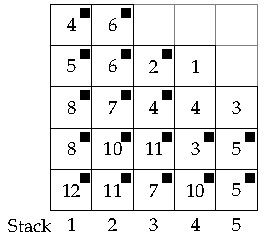
\includegraphics{figs/c.pdf}
\caption{Pre-extreme state.}
\label{fig:pre-extreme}
\end{figure}
Based on the above discussion, we can see that when $\sum_{s\in\mathbb{S}}f(s)<N-2$, there is a chance to generate dead-end state.

When the current state is a pre-extreme state, we eliminate the container--stack pairs $c\rightarrow s$ such that $f(s)=H-1$ from $\mathbb T$, so that the algorithm avoids entering a dead-end state.
\subsection{Task evaluation}
Every valid task $c\rightarrow s\in\mathbb{T}$ is evaluated by a tuple with six elements: the tier-protection indicator, the number of moves required by the STAP, the number of stable containers that need to be moved from the aim stack $sh(s)-f(s)$, the affected demand, fixed height of the aim stack $f(s)$, $-g(c)$.
The tuples of valid tasks are compared lexicographically, and the task with the minimum tuple is selected as the next task. The six elements in the tuple will be explained in the following.

The tier-protection indicator is to balance the trade-off between the freedom of task selection and the surplus loss. In principle, a container can be moved to any valid stack. But if a container with small group value occupies an (relatively) empty stack, then the loss of the surplus vector is large: after the target container $c$ is fixed to the target slot $(s,f(s)+1)$, the surplus $\Delta(\varphi)$ is reduced by $H-f(s)$, for $\varphi\in (g(c),g(s,f(s)]$. The larger the spread between $g(c)$ and $g(s,f(s))$ is, the more the surplus vector will lose. For example, in Figure \ref{fig:pre-extreme}, if container 1 (container with group value 1) is moved on container 3 (stack 5 tier 3), the supply of group 3 is reduced by 2 as 1 becomes the highest orderly container of stack 5. The cumulative supplies $G(3)$ and $G(2)$ are reduced by 2 accordingly.

If a pair $c\rightarrow s$ satisfies $f(s)<P1$ and affected demand $\sum_{\varphi=g(c)+1}^{g(s,f(s))}d(\varphi)\ge P2$, then the task cannot be carried out and is deleted from the evaluation list. As customizable parameters, the number of tiers protected $P1$ and the threshold value $P2$ can be adjusted optionally.

The number of moves required by the STAP is the movements for moving $c$ to $s$, the number is precise while in \cite{wang2015} the number is just an estimation. The process to calculate the number is introduced in Section \ref{sec:speedy}.
The affected demand is $\sum_{\varphi=g(c)+1}^{g(s,f(s))}d(\varphi)$.




\subsection{Speedy task accomplishment procedure}

\label{sec:speedy}
After the task is decided, a speedy task accomplishment procedure (STAP) is carried out to accomplish the task, resulting in a new state. STAP is a move sequence which is based on task types.

Let the target container be denoted by $c^*$ (located in $(s^+,t^+)$) and the target stack by $s^*$. The task is \emph{immediate} if $c^*$ is just on the highest fixed container in $s^*$, i.e., $s^+=s^*$ and $t^+=f(s^*)+1$; \emph{internal} if $c^*$ is above but not on the highest fixed container in $s^*$, i.e., $s^+=s^*$ and $t^+>f(s^*)+1$; and \emph{external} if $c^*$ and $s^*$ are in different stacks, i.e., $s^+\neq s^*$.


\subsubsection{Immediate task}

An immediate task does not require any move because the target container is already located in the target slot.

\subsubsection{Internal task}

For an internal task, let $a$ denote the number of empty slots except those in $s^+$ and the highest non-full stack; that is, $a=E-e(s^+)-\min\{e(s)>0: s\neq s^+\}$. If multiple stacks are with the maximum height, only one is excluded. Let $b_1$ and $b_2$ denote the numbers of blocking containers above and below $c^*$ in stack $s^+$, respectively. Blocking containers refer to those above target containers or target slots.
The accomplishment procedure of an internal task is given in Algorithm~\ref{algo:internal}.

\begin{algorithm*}[htbp]

\caption{Accomplish an internal task.}
\label{algo:internal}

\setalgo

\SetKwProg{One}{case I1:}{}{end~case}
\SetKwProg{Two}{case I2:}{}{end~case}
\SetKwProg{Three}{case I3:}{}{end~case}
\SetKwInput{Target}{target container}
\SetKwInput{Aim}{aim slot}
\SetKwInput{Above}{blocking above}
\SetKwInput{Below}{blocking below}
\SetKwInput{Slot}{slot supply}

\begin{multicols}{2}
\Target{$c^*(s^+,t^+)$}

\Aim{$(s^+,f(s^+)+1)$}
\Slot{$a=E-e(s^+)-\min\{e(s)>0: s\neq s^+\}$}

\Above{$b_1=h(s^+)-t^+$}
\Below{$b_2=t^+-f(s^+)-1$}
  \One{$a\ge b_2$}
  {
    \Repeat{$b_1$}
    {
      $\mathbb{R}\gets \{s\neq s^+: h(s)<H,\, \alpha(s^+,s)\ge b_2\}$\;

      \Relocate{$s^+,1,\mathbb{R}$}\;
    }
    $\mathbb{I}\gets \{s\neq s^+: h(s)<H,\, E-e(s^+)-e(s)\ge b_2\}$\;

    $\mts\gets \Interim{$\mathbb{I}$}$\;
    \Move{$s^+,1,s'$}\;
    \Relocate{$s^+,b_2,\mathbb{S}\setminus\{s^+,\mts\}$}\;
    \Move{$\mts,1,s^+$}\;
    \tcp{I1:\ $h(s^+)-f(s^+)+1$ moves}
  }

  \Two{$a<b_2$ \& $|\{s\neq s^+: h(s)<H\}|>1$}
  {
    \Relocate{$s^+, b_1, \mathbb{S}\setminus\{s^+\}$}\;
    $\mts_1\gets \Interim{$\mathbb{S}\setminus\{s^+\}$}$\;
    \Move{$s^+, 1, \mts_1$}\;
    $k_2\gets E-e(s^+)-e(\mts_1)-1$\;
    \Relocate{$s^+, k_2, \mathbb{S}\setminus\{s^+,\mts_1\}$}\;
    Find $\mts_2$ s.t.\ $\mts_2\not\in \{s^+,\mts_1\}$ \& $h(\mts_2)<H$\;
    \Move{$\mts_1, 1, \mts_2$}\;
    \Move{$s^+, b_2-k_2, \mts_1$}\;
    \Move{$\mts_2, 1, s^+$}\;
    \tcp{I2:\ $h(s^+)-f(s^+)+2$ moves}
  }

  \Three{$a<b_2$ \& $|\{s\neq s^+: h(s)<H\}|=1$}
  {
    Find $s'$ s.t.\ $s'\neq s^+$ \& $h(s')<H$\;
    $\mts\gets \InterimFull{$\mathbb{S}\setminus\{s^+,s'\}$}$\;\label{line:wholly}
    \BiSender{$\mts, 1, s^+, b_1, \{s'\}$}\;\label{line:dualsender}
    \Move{$s^+, 1, \mts$}\;
    \Move{$s^+, b_2, s'$}\;
    \Move{$\mts, 1, s^+$}\;
    \tcp{I3:\ $h(s^+)-f(s^+)+2$ moves}
  }

\end{multicols}
\BlankLine
\BlankLine
\end{algorithm*}

The accomplishment procedure is carried out based on the relationship between available empty slots and the number of blocking containers. The relationship determines how containers are relocated.
\begin{itemize}
\item I1: $a\ge b_2$;
\item I2: $a<b_2$ \& $|\{s\neq s^+: h(s)<H\}|>1$; and
\item I3: $a<b_2$ \& $|\{s\neq s^+: h(s)<H\}|=1$.
\end{itemize}

In case I1, $b_1$ containers above $c^*$ are relocated one by one. $\mathbb R$ represents the set of available destination stack for the top container which blocks $c^*$. A stack $s$ is available if $s\neq s^+,h(s)<H,\alpha(s^+,s)\ge b_2$. Here $\alpha$ function in Algorithm \ref{algo:alpha} indicates how many slots are left for $b_2$.


\begin{algorithm}[htbp]

\caption{Alpha function.}
\label{algo:alpha}
\setalgo
\begin{multicols}{2}
\Function{$\alpha(s^+,\mds)$}
        {\tcp{$s^+\neq \mds$}
            $e^{\min}\gets \min\{e(s)>0:s\neq s^+\}$\;
            $e^{\sec}\gets \min\{e(s)>e^{\min}:s\neq s^+\}$\;
            $k^{\min}\gets |\{s\neq s^+ : e(s)=e^{\min}\}|$\;
            \uIf{$e(\mds)> e^{\min}$}
            {
                \Return $E-e(s^+)-e^{\min}-1$\;
            }
            \uElseIf{$e^{\min}\ge 2$}
            {
                \Return $E-e(s^+)-e^{\min}$\;
            }
            \uElseIf{$k^{\min}=1$}
            {
                \Return $E-e(s^+)-e^{\sec}-1$\;
            }
            \Else
            {
                \Return $E-e(s^+)-2$\;
            }
        }
\end{multicols}
\end{algorithm}
In the process of relocating containers from $b_1$, it need consider reserving slots for containers from $b_2$. Because $c^*$ is above $b_2$. After retrieving $b_1$, $c^*$ is relocated before containers in $b_2$.
If the relocation is to put $c^*$ and $b_2$ in the same stack, then $c^*$ needs additional moves to be retrieved. Hence, we reserve the stack with the minimum empty slots $s_{\text{min}}$ for $c^*$, and the slots from $\{s\in S: s\neq s^+, s\neq s_\text{min}\}$ for $b_2$.
Of course, containers in $b_1$ can also occupy $s_\text{min}$ and $\{s\in S: s\neq s^+, s\neq s_\text{min}\}$, and definitely $|\{s\in S: s\neq s^+\}|\ge b_1+b_2$. But the number of containers from $b_1$ which occupy $\{s\in S: s\neq s^+, s\neq s_\text{min}\}$ needs computation, in order to satisfy $b_2$ first. Hence, when deciding whether a stack $s^{\text{dst}}$ can be the destination of a container $c$ from $b_1$, $\alpha$ function is used to compute if $c$ is placed to $s^{\text{dst}}$ how many slots left for $b_2$. And if the left slots are not enough for $b_2$, $c$ cannot be moved to $s^{\text{dst}}$.

If $e(\mds)> e^{\min}$, that is, $\mds$ is not the highest non-full stack. $e^{\min}$ is reserved for $c^*$. Slots of $s^+$ cannot be used. If $c$ is moved to $\mds$, left slots for $b_2$ is $E-e(s^+)-e^{\min}-1$.

If $e(\mds)=e^{\min}\ge 2$, that is $\mds$ is the highest non-full stack and it has at least 2 empty slots. If $c$ is moved to $e(\mds)$, the stack can also accommodate $c^*$, hence, left slots for $b_2$ is $E-e(s^+)-e^{\min}$.

If $e(\mds)=e^{\min}=1$ and $k^{\min}=1$, that is, $\mds$ is the unique highest stack with only one empty slot. If $c$ is moved to $s^{\mds}$, the stack with the second highest height will reserve for $c^*$ in the next round. The slots left for $b_2$ becomes $E-e(s^+)-e^{\text{sec}}-1$.

If $e(\mds)=e^{\min}=1$ and $k^{\min}\ge2$, another stack with the one empty slot accommodates $c^*$ in the future. If $c$ is moved to $s^{\mds}$, the slots left for $b_2$ becomes $E-e(s^+)-2$.

The container relocation is illustrated in Algorithm~\ref{algo:relocation}, which relocates $k$ containers from a {sender} stack $\mss$ to $\mathbb R$. For each of the top $k$ containers of the sender, the destination stack $\mds$ is properly selected from $\mathbb{R}$ according to the evaluations by function \EvalMove{$\mss,\mds$}. Function \Move{$\mss,k,\mds$} performs $k$ relocations from stack $\mss$ to stack $\mds$. The function \EvalMove{$\mss,\mds$} and \Move{$\mss,k,\mds$} are also illustrated in Algorithm~\ref{algo:relocation}.


\begin{algorithm}[htbp]

\caption{Relocation function.}
\label{algo:relocation}
\setalgo
\begin{multicols}{2}


\Function{\Relocate{$\mss,k,\mathbb{R}$}}
{
  \Repeat{k}
  {
    $\mathbb{R}'\gets \{s\in \mathbb{R}:h(s)<H\}$\;
    $\mds\gets \arg\min_{s\in\mathbb{R}'} \EvalMove{$\mss,s$}$\;
    \Move{$\mss,1,\mds$}\;
  }
}
\Function{\Move{$\mss,k,\mds$}}
{
  Move $k$ containers from stack $\mss$ to stack $\mds$\;

}

\Function{\EvalMove{$\mss,\mds$}}
{
  $c\gets (\mss,h(\mss))$\;
  $g\gets g(c)$\;
  $q\gets q(\mds,h(\mds))$\;
  \uCase{$ sh(\mds)=h(\mds)$ \& stack $\mds$ can stabilize $c$}
  {
    \Return $\langle1, \sum_{\varphi=g+1}^q d(\varphi)\rangle$\;
  }
  \uCase{$ sh(\mds)<h(\mds)$ \& $g\ge m(\mds)$}
  {
    \Return $\langle2,g-m(\mds)\rangle $\;
  }
  \uCase{$ g(\mds)<h(\mds)$ \& $g<m(\mds)$}
  {
    \Return $\langle3, m(\mds)-g \rangle$\;
  }
  \Case{$ g(\mds)=h(\mds)$ \& stack $s_2$ cannot stabilize $c$}
  {
    \Return $\langle 4,q \rangle$\;
  }
}
\end{multicols}
\end{algorithm}
Let us define the capability of an occupied slot $(s,t)$ by $q(s,t) = g(s, t)$ if the container inside is orderly, otherwise $q(s, t) = 0$; specifically, regarding the ground as an occupied slot at tier 0 with group value G. %Thus, we can easily verify the placement of a container (s; t) by checking whether p(s; t)  q(s; t ?? 1).
The evaluations of moves are represented by numerical tuples, which are lexicographically comparable. \EvalMove{$\mss,\mds$} returns the penalty of the move from stack $\mss$ to $\mds$. Define the \emph{messiness} of stack $s$ by $m(s)=\max_{sh(s)<t\le h(s)}g(s,t)$, that is the largest group value among the unstable containers in stack $s$. The preferences of selecting a stack $\mds$ as the destination stack for a blocking container are as follows.
\begin{enumerate}
\item If stack $\mds$ is entirely stable and can stabilize $c$, the minimum affected demand is preferred;
\item If stack $\mds$ is not entirely stable and $g(c)\ge m(\mds)$, the minimum gap between $m(\mds)$ and $g(c)$ is preferred;
\item If stack $\mds$ is not entirely stable and $g(c)> m(\mds)$, the minimum gap between $g(c)$ and $m(\mds)$ is preferred;
\item If stack $\mds$ is entirely stable but cannot stabilize $c$, the minimum $q(\mds,h(\mds))$ is preferred.
\end{enumerate}

The first preference indicates that stabilizing a blocking container reduces the total number of unstable containers in the bay. The second and third preferences consider the messiness of the destination stack. Messiness refers to the largest group value of the unstable containers in a stack; larger messiness implies a higher urgency of reshuffles. The last preference indicates that an entirely stable stack should be protected from being ruined.

Function \EvalMove returns a tuple, the first element indicates the type of the value and the second element indicates the scale of the value.

In cases I1 and I2, an interim stack is selected to temporarily store the target container (function \Interim{$\mathbb{I}$}).
The selection prefers stacks that are not entirely stable, with the largest messiness, then entirely stable stacks with the smallest group of orderly containers. The most unattractive stack for receiving blocking containers is selected as the interim stack. In cases I3 and E4 (in Section~\ref{sec:external}), the interim stack is selected by the minimum group value of the top containers of these full stacks, which is function \InterimFull{$\mathbb{F}$}.

\begin{algorithm}[htbp]

\caption{Interim and InterimFull functions.}
\label{algo:interim}
\setalgo
\begin{multicols}{2}
\Function{\Interim{$\mathbb{I}$}}
{
  $\mathbb{I}_1\gets \{s\in \mathbb{I}:  sh(s)<h(s)<H\}$\;
  $\mathbb{I}_2\gets \{s\in \mathbb{I}:  sh(s)=h(s)<H\}$\;

  \uIf{$\mathbb{I}_1\neq \varnothing$}
  {
    \Return $\arg\max_{s\in\mathbb{I}_1} m(s)$\;
  }
  \Else
  {
    \Return $\arg\min_{s\in\mathbb{I}_2} q(s,h(s))$\;
  }

}




\Function{\InterimFull{$\mathbb{F}$}}
{
  $\mathbb{F}_1\gets \{s\in \mathbb{F}: f(s)\le sh(s)<h(s)=H\}$\;
  $\mathbb{F}_2\gets \{s\in \mathbb{F}: f(s)< sh(s)=h(s)=H\}$\;
  \uIf{$\mathbb{F}_1\neq \varnothing$}
  {
    \Return $\arg\min_{s\in\mathbb{F}_1} g(s,h(s))$\;
  }
  \Else
  {
    \Return $\arg\min_{s\in\mathbb{F}_2} g(s,h(s))$\;
  }
}

\end{multicols}
\end{algorithm}

Function \BiSender{$\mss_1,k_1,\mss_2,k_2,\mathbb{R}$} performs relocations from two senders, stacks $\mss_1$ and $\mss_2$, to the same receiver set $\mathbb{R}$, and the respective quantities are $k_1$ and $k_2$. The moving order of the two top containers from two senders is determined by the evaluation tuple. The one with smaller tuple is moved first. In Algorithm~\ref{algo:bisender}, $\vec{v}_1$ and $\vec{v}_2$ are tuple results of function \EvalMove.

Likewise, function \BiReceiver{$\mss,k_1,\mathbb{R}_1,k_2,\mathbb{R}_2$} in the external case relocates $k_1$ and $k_2$ containers from one sender stack $\mss$ to two receiver sets, $\mathbb{R}_1$ and $\mathbb{R}_2$, respectively.

\begin{algorithm}[htbp]

\caption{BiSender and BiReceiver functions.}
\label{algo:bisender}
\setalgo


\begin{multicols}{2}
\Function{\BiSender{$\mss_1,k_1,\mss_2,k_2,\mathbb{R}$}}
{
  $i\gets k_1$, $j\gets k_2$\;
  \Repeat{$k_1+k_2$}
  {
    \uIf{$j=0$}{
      \Relocate{$\mss_1,i,\mathbb{R}$}\;
      $i\gets 0$\;
    }
    \uElseIf{$i=0$}{
      \Relocate{$\mss_2,j,\mathbb{R}$}\;
      $j\gets 0$\;
    }
    \Else
    {
      $\mathbb{R}'\gets \{s\in \mathbb{R}:h(s)<H\}$\;
      $\mds_1\gets \arg\min_{s\in\mathbb{R}'} \EvalMove{$\mss_1,s$}$\;
      $\vec{v}_1\gets \EvalMove{$\mss_1,\mds_1$}$\;
      $\mds_2\gets \arg\min_{s\in\mathbb{R}'} \EvalMove{$\mss_2,s$}$\;
      $\vec{v}_2\gets \EvalMove{$\mss_2,\mds_2$}$\;
      \eIf{$\vec{v}_1\le^{\mathrm{lex}} \vec{v}_2$}
      {
        \Move{$\mss_1,1,\mds_1$}\;
        $i\gets i-1$;
      }
      {
        \Move{$\mss_2,1,\mds_2$}\;
        $j\gets j-1$\;
      }
    }
  }
}
%\Function{\MoveNeed{$c,s$}}
%{
%  \uIf{$(c,s)$ is immediate}
%  {
%    \Return 0\;
%  }
%  \Else
%  {
%    \Return actual number of moves needed by the STAP to accomplish the task $(c,s)$\;
%    }
%}
\Function{\BiReceiver{$\mss,k_1,\mathbb{R}_1,k_2,\mathbb{R}_2$}}
{
  $i\gets k_1$, $j\gets k_2$\;
  \Repeat{$k_1+k_2$}
  {
    \uIf{$j=0$}{
      \Relocate{$\mss,i,\mathbb{R}_1$}\;
      $i\gets 0$\;
    }
    \uElseIf{$i=0$}
    {
      \Relocate{$\mss,j,\mathbb{R}_2$}\;
      $j\gets 0$\;
    }
    \Else
    {
      $\mathbb{R}_1'\gets \{s\in \mathbb{R}_1:h(s)<H\}$\;
      $\mathbb{R}_2'\gets \{s\in \mathbb{R}_2:h(s)<H\}$\;


      $\mds_1\gets \arg\min_{s\in\mathbb{R}_1'} \EvalMove{$\mss,s$}$\;
      $\vec{v}_1\gets \EvalMove{$\mss,\mds_1$}$\;
      $\mds_2\gets \arg\min_{s\in\mathbb{R}_2'} \EvalMove{$\mss,s$}$\;
      $\vec{v}_2\gets \EvalMove{$\mss,\mds_2$}$\;

      \eIf{$\vec{v}_1\le^{\mathrm{lex}}\vec{v}_2$}
      {
        \Move{$\mss,\mds_1$}\;
        $i\gets i-1$\;
      }
      {
        \Move{$\mss,\mds_2$}\;
        $j\gets j-1$\;
      }
    }
  }
}

\end{multicols}

\BlankLine
\BlankLine
\end{algorithm}

The total number of moves needed in case I1 is $h(s^+)-f(s+)+1$, and the number of moves in case I2 and case I3 is $h(s^+)-f(s+)+2$. All are noted in the comment of Algorithm~\ref{algo:internal}.

Note that in case I2, the target container $c^*$ is moved to the new interim stack $\mts_2$ from the first interim stack $\mts_1$ when there is only one empty slot remaining in $\mathbb{S}\setminus\{s^+,\mts_1\}$. This can be modified so that $c^*$ can be moved to a new interim stack $\mts_2$ earlier as long as the empty slots in $\mathbb{S}\setminus\{s^+,\mts_2\}$ are enough for the remaining blocking containers in stack $s^+$. Moreover, if there is a full stack in $\mathbb{S}\setminus\{s^+\}$ in case I2, the task can also be completed in a similar way as that used in case I3, with the same operational cost.

\subsubsection{External task}
\label{sec:external}
For an external task, the number of empty slots in $\mathbb{S}\setminus\{s^+,s^*\}$ is denoted by $a$; that is, $a=E-e(s^+)-e(s^*)$. Let $b_1$ and $b_2$ denote the numbers of blocking containers above the target container $c^*$ and the aim slot $(s^*,f(s^*))$, respectively. The pseudo-code describing the accomplishment for an external task is given in Algorithm~\ref{algo:external}, with four situations considered,\begin{itemize}
\item E1: $a\ge b_1+b_2$;
\item E2: $b_1+1\le a<b_1+b_2$;
\item E3: $1\le a<b_1+\min\{1,b_2\}$; and
\item E4: $a=0<b_1+b_2$.
\end{itemize}



\begin{algorithm*}[htbp]
\caption{Accomplish an external task.}
\label{algo:external}

\setalgo

\SetKwProg{One}{case E1:}{}{end~case}
\SetKwProg{Two}{case E2:}{}{end~case}
\SetKwProg{Three}{case E3:}{}{end~case}
\SetKwProg{Four}{case E4:}{}{end~case}
\SetKwInput{Target}{target container}
\SetKwInput{Aim}{aim slot}
\SetKwInput{BPlus}{blocking above target}
\SetKwInput{BMinus}{blocking in aim stack}
\SetKwInput{Slot}{slot supply}


\begin{multicols}{2}

\Target{$c^*(s^+,t^+)$}
\Aim{$(s^*,f(s^*)+1)$}
\BPlus{$b_1=h(s^+)-t^+$}
\BMinus{$b_2=h(s^*)-f(s^*)$}
\Slot{$a=E-e(s^+)-e(s^*)$}

  \One{$a\ge b_1+b_2$}
  {
    \BiSender{$s^+, b_1,s^*,b_2, \mathbb{S}\setminus\{s^+,s^*\}$}\;
    \Move{$s^+, 1, s^*$}\;
    \tcp{E1:\ $b_1+b_2+1$ moves}
  }

  \Two{$b_1+1\le a<b_1+b_2$}
  {
    $k_2\gets a-1-b_1$\;
    \BiSender{$s^+, b_1, s^*, k_2, \mathbb{S}\setminus\{s^+,s^*\}$}\;
    Find $\mts$ s.t.\ $\mts\not\in \{s^+,s^*\}$ \& $h(\mts)<H$\;
    \Move{$s^+,1,\mts$}\;
    \Move{$s^-, b_2-k_2, s^+$}\;
    \Move{$\mts, 1, s^*$}\;
    \tcp{E2:\ $b_1+b_2+2$ moves}
  }


  \Three{$1\le a<b_1+\min\{1,b_2\}$}
  {
    $k_1\gets a-1$\;
    \BiReceiver{$s^+, k_1, \mathbb{S}\setminus\{s^+,s^*\}, b_1-k_1, \{s^*\}$}\;\label{line:dualreceiver}
    Find $\mts$ s.t.\ $\mts\not\in \{s^+,s^*\}$ \& $h(\mts)<H$\;
    \Move{$s^+,1,\mts$}\;
    \Move{$s^*, b_1-k_1+b_2, s^+$}\;
    \Move{$\mts, 1, s^*$}\;
    \tcp{E3:\ $2b_1+b_2-a+3$ moves}
  }

  \Four{$a=0<b_1+b_2$}
  {
    $\mts\gets \InterimFull{$\mathbb{S}\setminus\{s^+,s^*\}$}$\;\label{line:fixed}
    \BiSender{$\mts, 1, s^+, b_1, \{s^*\}$}\;
    \Move{$s^+, 1, \mts$}\;
    \Move{$s^*, b_1+b_2+1, s^+$}\;
    \Move{$\mts, 1, s^*$}\;
    \tcp{E4:\ $2b_1+b_2+4$ moves}
  }

\end{multicols}

\BlankLine
\BlankLine
\end{algorithm*}


%\subsection{Common functions}
%\label{sec:commonfunction}









%\subsubsection{Regression issue}
%\label{sec:reg}
%
%In cases I3 and E4, if the top container of the full stack selected (cf.\ line~\ref{line:wholly} in Algorithm~\ref{algo:internal} and line~\ref{line:fixed} in Algorithm~\ref{algo:external}) is not fixed, the task is done without any side effect. However, if the top container has been fixed, the container should be returned to its previously fixed slot, requiring additional moves.
%
%The regression issue only occurs in tricky states, and it can be avoided if the tricky state avoidance technique (cf.\ Section~\ref{sec:avoid}) is applied.

%The proposed {greedy and speedy heuristic} (GASH) is a realized implementation of the generic feasibility-based heuristic scheme.
%The GASH employs all the techniques introduced above, i.e., the container stability concept, the techniques of tricky state avoidance and bottom tiers protection, and the STAP\@. The procedure of the GASH and the user-defined functions for the STAP are given in Algorithm~\ref{algo:gash}.



%\begin{algorithm*}[htbp]
%\caption{Greedy and speedy heuristic.}
%\label{algo:gash}
%
%
%\setalgo
%
%
%\begin{multicols}{2}
%\Begin
%{
%  $(\mathsf{L},\boldsymbol{f})\gets (\mathsf{L}^0,U\cdot\boldsymbol{1})$\;
%  \Repeat{$N-SU$}
%  {
%    $\mathbb{T}\gets \Valid{}$\;
%    $(c^*, s^-)\gets \arg\min_{(c,s)\in\mathbb{T}} \EvalTask{$c,s$}$\;
%    Accomplish $( c^*, s^-)$ by the STAP\;
%    $f(s^-)\gets f(s^-)+1$\;
%  }
%}
%
%\Function{\Valid{}}
%{
%  $\mathbb{T}\gets \varnothing$\;
%
%  \ForEach{$(c,s)\in\mathbb{C}\times\mathbb{S}$}
%  {
%      \If{$c$ is unfixed \\\& $f(s)<H$ \\\& $p(c)\le q^f(s)$ \\\& $\Delta(\varphi)\ge H-f(s)$, for $p(c)< \varphi\le q^f(s)$}
%      {
%        $\mathbb{T}\gets \mathbb{T}\cup\{(c,s)\}$\;
%      }
%  }
%  \Return $\mathbb{T}$\;
%}
%
%
%
%\Function{\EvalTask{$c,s$}}
%{
%  $p\gets p(c)$\;
%  $q\gets q^f(s,f(s))$\;
%  $\chi\gets 0$ \tcp*[l]{key indicator}
%  \If{$f(s)<2$ \& $\delta(p,q)\ge S$}
%  {
%    \tcp{bottom tiers protection}
%    $\chi\gets \infty$\;
%  }
%  \If{$(\mathsf{L},\boldsymbol{f})$ is pre-tricky \& $f(s)=H-1$}
%  {
%    \tcp{tricky state avoidance}
%    $\chi\gets \infty$\;
%  }
%
%  $n\gets \MoveNeed{$c,s$}$\;
%
%  \Return $\langle \chi,\ n,\  g(s)-f(s),\ \delta(p,q),\ f(s),\ -p(c) \rangle$\;
%}
%
%
%
%
%
%\end{multicols}
%\BlankLine
%\BlankLine
%\end{algorithm*}



%Function \Valid{} returns $\mathbb{T}$, the set of valid tasks for the current state.


%Note that because the tricky state avoidance technique is applied, the regression issue would never happen in the GASH, although it is still considered in function \InterimFull{$\mathbb{F}$} to complete the whole logic.

\section{Computational results}
\label{sec:experiment}

In this section, the proposed feasibility-based heuristic (FBH) is compared to two benchmark heuristic approaches. One is the target-guided heuristic (TGH) proposed in our previous work \citep{wang2015}, and the other is a similar implementation to the LPFH proposed by \cite{exp2012}. Since the LPFH only discusses cases with enough empty slots (cases I1 and E1 in our statement) and involves random decisions, it is difficult to implement a deterministic version. Thus, we developed a substitute instead, referred to as the largest group value first heuristic (LGVFH). We implemented both TGH and LGVFH. Experiments were conducted on a PC with Intel Core i7 CPU clocked at 3.40 GHz with Windows 7 operating system. The code was written in Java.

The LGVFH selects the next target container from unfixed containers with the largest group value, and then accomplish it by the STAP with the same user-defined functions used as that in the FBH\@. Necessary pseudo-code for the LGVFH is given in Algorithm~\ref{algo:lpvfh}.

\begin{algorithm*}[htbp]
\caption{Largest group value first heuristic.}
\label{algo:lpvfh}


\setalgo

\begin{multicols}{2}

\Begin
{
  $(\mathsf{L},\boldsymbol{f})\gets (\mathsf{L}^0,U\cdot\boldsymbol{1})$\;

  \ForEach{$g=G,\dots,1$}
  {
    $\mathbb{C}_g\gets\textrm{containers with group value $g$}$\;
    $\mathbb{A}_g\gets\varnothing$\tcp*[l]{set of aim stacks}
    \While{$\mathbb{C}_g\neq \varnothing$}
    {
      $(c^*, s^*)\gets \arg\min_{c\in\mathbb{C}_g, f(s)<H} \MoveNeed{$c,s$}$\;
      Accomplish $( c^*, s^-)$ by the STAP\;
      $f(s^*)\gets f(s^*)+1$\;
      $\mathbb{C}_g\gets\mathbb{C}_g\setminus\{c^*\}$\;
      $\mathbb{A}_g\gets \mathbb{A}_g\cup \{s^*\}$\;
    }
    \ForEach{$s^*\in\mathbb{A}_g$}
    {
    	\Fill{$s^*$}\;
    }
  }
}



\Function{\Fill{$s$}}
{
  \While{$h(s)<H$}
  {
    $\mathbb{S}'\gets\varnothing$\;
    \ForEach{$i\in\{i\neq s: sh(i)<h(i)\}$}
    {
      $c\gets (i,h(i))$\;
      \If{ stack $s$ can stabilize $c$}
      {
        $\mathbb{S}'\gets \mathbb{S}'\cup \{i\}$\;
      }
    }
    \eIf{$\mathbb{S}'\neq \varnothing$}
    {
      $s'\gets \arg\max_{i\in\mathbb{S}'} g(i,h(i))$\;
      \Move{$s',1,s$}\;
    }
    {
      \Break\;
    }
  }
}
\end{multicols}
\BlankLine
\BlankLine
\end{algorithm*}

Here, function \MoveNeed{$c,s$} is the actual number of moves needed by the STAP to accomplish the task $(c,s)$. Function \Fill{$s$} is achieved by fulfilling $s$ with those unstable containers in other stacks which $s$ stabilizes.



The problem instance format of the CPMP is the same as that of the {container relocation problem} (CRP, a.k.a.\ the blocks relocation problem), the problem of minimizing the total number of container moves for retrieving containers from the initial layout.
In the literature, researchers usually use the same data sets when solving the CPMP~\citep{bort2012,cas2009,exp2012,wang2015} and the CRP~\citep{cas2011,exp2014,forster2012,jin2013,jin2015}.

\subsection{Configuration of P1 and P2}
This section shows the effect of the tier-protection indicator. We selected six settings of the two parameters $(P1,P2$), which is $(0,N), (H/4,N/2), (H/3,N/6), (2H/3,N/8), (H,N/10)$. We made $P1 (P2)$ proportional to $H (N)$, since $f(s)$ (affected demand) is related to height (number of containers).

The six settings are in a loose-intermediate-tight order, and algorithms will filter out more tasks when using back settings. The result is shown in Table~\ref{tab:tier-protection}. The first column indicates the parameter setting. The second and third columns indicate the average movements of CVS and BF data sets, respectively. Parameter $(0,N)$ means that there is no tier-protection indicator as no task is filtered out. As the setting becomes tight, the performance of both CVS and BF is improved, until a peak is achieved. But when the setting becomes extremely tight, the performance decreases. When the setting is $(H,N/10)$, some instances of CVS even cannot find a solution; therefore, we make the unit with ``Nil''. The instances of BF are loose, that is, the empty slots are sufficient. Solutions can be found even if under setting $(H,N/10)$, but the performance is worse than that with intermediate setting.
\begin{table}[htbp]
  \centering
  \caption{Configuration of $P1$ and $P2$}
    \begin{tabular}{lrr}
    \toprule
    $(P1,P2)$ & CVS   & BF \\
    \midrule
    $(0,N)$   & 52.15 & 71.69 \\
    $(H/4,N/2)$ & 50.43 & 71.21 \\
    $(H/3,N/4)$ & 45.82 & 69.05 \\
    $(H/2,N/6)$ & 45.32 & 69.51 \\
    $(2H/3,N/8)$ & 46.33 & 71.23 \\
    $(H,N/10)$ & Nil   & 73.44 \\
    \bottomrule
    \end{tabular}%
  \label{tab:tier-protection}%
\end{table}%



\subsection{Results for CVS instances}

\citet{cas2011} present the complete CVS data set (named after the authors' surnames, Caserta, Vo{\ss} and Sniedovich) originally for the CRP\@. The CVS instances are classified into 21 groups, each consisting of 40 instances. The stacks of the initial layout have the same height in a CVS instance. The number of containers per stack in the initial layout is denoted by $K$, hence $N=SK$. It is worth noting that the stack height limitation is not specified in the original data. The researchers add two extra tiers above the initial layout; that is, $H=K+2$.

The CVS instances can be considered typical dense CPMP instances. Table~\ref{tab:cvs} illustrates the computational results on CVS instances by the TGH, the LGVFH, and the FBH\@. The values under the ``move'' headings represent average number of moves for every CVS group, whereas the values under the ``time (ms)'' headings are the run time in ms. The values under the ``improvement'' heading are the improvements compared to TGH and LGVFH in percentage.
The results showcase that the FBH surpasses the benchmark heuristics by more than $10\%\times N$ moves on most instance groups. Especially on the narrowest group CVS~10-6, the FBH outperforms the TGH and the LGVFH by 319.38\% and 55.54\%, respectively.

\begin{table}[htbp]
\caption{Results for CVS instances.}
\label{tab:cvs}

%\settab

\centering
\begin{tabular}{ccccccccc}
\toprule
\multirow{2}{*}{CVS~K-S}&

\multicolumn{2}{@{}c@{}}{TGH}
&
\multicolumn{2}{@{}c@{}}{LGVFH}
&
\multicolumn{2}{@{}c}{FBH}
&
\multicolumn{2}{@{}c@{}}{improvement}\\

\cmidrule{2-3}
\cmidrule{4-5}
\cmidrule{6-7}
\cmidrule{8-9}
          & move&time (ms)&move    &time (ms)& move&  time (ms) &TGH & LGVFH \\
\midrule
CVS 3-3   & 12.95  & 0.43 & 11.25  & 0.45 & 11.28  & 0.53       & 12.93\%   & -0.22\%\\
CVS 3-4   & 12.18  & 0.20 & 12.23  & 0.15 & 10.80  & 0.18       & 11.29\%   & 11.66\%\\
CVS 3-5   & 12.78  & 0.10 & 13.45  & 0.20 & 12.08  & 0.18       & 5.48\%    & 10.22\%\\
CVS 3-6   & 14.38  & 0.18 & 14.88  & 0.33 & 12.98  & 0.23       & 9.74\%    & 12.77\%\\
CVS 3-7   & 16.00  & 0.13 & 16.58  & 0.23 & 14.75  & 0.15       & 7.81\%    & 11.01\%\\
CVS 3-8   & 16.55  & 0.15 & 17.08  & 0.28 & 15.65  & 0.38       & 5.44\%    & 8.35\%\\
CVS 4-4   & 23.35  & 0.05 & 21.93  & 0.08 & 21.88  & 0.15       & 6.32\%    & 0.23\%\\
CVS 4-5   & 26.73  & 0.10 & 26.48  & 0.18 & 23.08  & 0.18       & 13.66\%   & 12.84\%\\
CVS 4-6   & 27.58  & 0.08 & 27.20  & 0.23 & 24.75  & 0.48       & 10.24\%   & 9.01\%\\
CVS 4-7   & 29.93  & 0.08 & 31.23  & 0.38 & 27.63  & 0.10       & 7.69\%    & 11.53\%\\
CVS 5-4   & 44.83  & 0.08 & 35.83  & 0.18 & 35.08  & 0.08       & 21.75\%   & 2.09\%\\
CVS 5-5   & 42.40  & 0.05 & 36.50  & 0.25 & 35.33  & 0.23       & 16.69\%   & 3.22\%\\
CVS 5-6   & 50.63  & 0.13 & 43.08  & 0.23 & 39.88  & 0.23       & 21.24\%   & 7.43\%\\
CVS 5-7   & 48.83  & 0.13 & 46.95  & 0.73 & 41.68  & 0.28       & 14.64\%   & 11.24\%\\
CVS 5-8   & 56.68  & 0.20 & 51.83  & 0.63 & 47.50  & 0.48       & 16.19\%   & 8.35\%\\
CVS 5-9   & 57.50  & 0.08 & 55.65  & 1.08 & 50.45  & 0.90       &
12.26\%   & 9.34\%\\
CVS 5-10  & 62.80  & 0.53 & 60.88  & 1.30 & 54.63  & 0.80       & 13.02\%   & 10.27\%\\
CVS 6-6   & 74.33  & 0.13 & 57.85  & 0.28 & 55.23  & 0.50       &
25.7\%    & 4.54\%\\
CVS 6-10  & 88.63  & 0.43 & 79.73  & 1.88 & 75.60  & 1.65       & 14.7\%    & 5.17\%\\
CVS 10-6  & 332.25 & 0.30 & 173.95 & 1.08 & 140.63 & 0.85       & 57.57\%   & 19.16\%\\
CVS 10-10 & 302.90 & 0.90 & 190.50 & 5.05 & 179.23 & 3.65       & 40.83\%   & 5.92\% \\[\defaultaddspace]
Average   & 64.48  & 0.21 & 48.81  & 0.72 & 44.29  & 0.58       & 16.44\%   & 8.29\%\\
\bottomrule
\end{tabular}
\end{table}

\subsection{Results for BF instances}

\citet{bort2012} introduce 32 groups of CPMP instances (referred to as BF instances), each group consisting of 20 instances. In BF instances, the bay size is $S=16$ or $20$ and $H=5$ or $8$. The number of containers $N$ is either $0.6\times SH$ or $0.8\times SH$, the number of groups $G$ is either $0.2\times N$ or $0.4\times N$, and the number of disorderly containers $B$ is either $0.6\times N$ or $0.75\times N$ in the initial layout.

The BF instances can be considered typical loose CPMP instances. Table~\ref{tab:bf} illustrates the computational results on BF instances by the three heuristics. The values under the ��move�� headings represent average number of moves for every BF group, whereas
the values under the ��time (ms)�� headings are the run time in ms. The values under the ��improvement�� heading are the improvements compared to TGH and LGVFH in percentage.

\begin{table}[htbp]
\caption{Results for BF instances.}
\label{tab:bf}

\settab

\centering

\begin{tabular}{cccccccccccccc}
\toprule
\multirow{2}{*}[-.5\defaultaddspace]{BF}&
\multirow{2}{*}[-.5\defaultaddspace]{S}   &
\multirow{2}{*}[-.5\defaultaddspace]{H}    &
\multirow{2}{*}[-.5\defaultaddspace]{N}   &
\multirow{2}{*}[-.5\defaultaddspace]{G}    &
\multirow{2}{*}[-.5\defaultaddspace]{B}   &
\multicolumn{2}{@{}c@{}}{TGH} & \multicolumn{2}{@{}c@{}}{LGVFH} &\multicolumn{2}{@{}c}{FBH} &\multicolumn{2}{@{}c@{}}{improvement}\\
\cmidrule{7-8}
\cmidrule{9-10}
\cmidrule(r){11-12}
\cmidrule{13-14}
       &  & &   &  &   & move & time (ms) &move & time (ms) & move & time (ms)     & TGH & LGVFH\\
\midrule

1       & 16 & 5 & 48  & 10 & 29 & 29.10  & 2.85 & 29.55  & 5.05  & 29.15  & 4.80  & -0.17\% &1.35\%\\
2       & 16 & 5 & 48  & 10 & 36 & 36.00  & 1.35 & 36.60  & 2.90  & 36.00  & 3.65  & 0       & 1.64\%\\
3       & 16 & 5 & 48  & 20 & 29 & 29.45  & 0.85 & 30.90  & 2.65  & 29.35  & 3.30  & 0.34\%  & 5.02\%\\
4       & 16 & 5 & 48  & 20 & 36 & 36.00  & 0.55 & 37.20  & 1.55  & 36.15  & 1.60  & -0.42\% & 2.82\%\\
5       & 16 & 5 & 64  & 13 & 39 & 48.50  & 1.55 & 53.00  & 2.90  & 46.30  & 2.65  & 4.54\%  & 12.64\%\\
6       & 16 & 5 & 64  & 13 & 48 & 57.55  & 0.95 & 62.85  & 3.45  & 55.50  & 2.65  & 3.56\%  & 11.69\%\\
7       & 16 & 5 & 64  & 26 & 39 & 53.55  & 0.85 & 57.15  & 3.10  & 49.95  & 2.25  & 6.72\%  & 12.6\%\\
8       & 16 & 5 & 64  & 26 & 48 & 60.00  & 0.80 & 66.90  & 2.90  & 57.60  & 2.40  & 4\%     & 13.9\%\\
9       & 16 & 8 & 77  & 16 & 47 & 60.35  & 1.55 & 62.15  & 4.35  & 56.30  & 3.90  & 6.71\%  & 9.41\%\\
10      & 16 & 8 & 77  & 16 & 58 & 62.15  & 7.90 & 69.50  & 4.65  & 61.55  & 3.85  & 0.97\%  &11.44\%\\
11      & 16 & 8 & 77  & 31 & 47 & 61.25  & 1.15 & 63.70  & 4.20  & 55.00  & 3.35  & 10.2\%  & 13.66\%\\
12      & 16 & 8 & 77  & 31 & 58 & 63.45  & 1.10 & 68.50  & 4.15  & 61.45  & 3.30  & 3.15\%  & 10.29\%\\
13      & 16 & 8 & 103 & 21 & 62 & 107.45 & 1.75 & 110.85 & 6.45  & 96.50  & 5.55  & 10.19\% & 12.95\%\\
14      & 16 & 8 & 103 & 21 & 78 & 124.75 & 2.55 & 134.90 & 5.95  & 116.05 & 4.75  & 6.97\%  & 13.97\%\\
15      & 16 & 8 & 103 & 42 & 62 & 110.60 & 2.90 & 110.40 & 9.45  & 99.45  & 6.50  & 10.08\% & 9.92\%\\
16      & 16 & 8 & 103 & 42 & 78 & 133.35 & 1.55 & 137.40 & 7.40  & 115.45 & 5.85  & 13.42\% & 15.98\%\\
17      & 20 & 5 & 60  & 12 & 36 & 36.50  & 0.90 & 37.35  & 2.30  & 36.50  & 2.15  & 0       & 2.28\%\\
18      & 20 & 5 & 60  & 12 & 45 & 45.00  & 0.80 & 45.00  & 2.15  & 45.20  & 1.90  & -0.44\% & -0.44\%\\
19      & 20 & 5 & 60  & 24 & 36 & 36.80  & 0.75 & 38.50  & 2.90  & 36.75  & 1.95  & 0.14\%  & 4.55\%\\
20      & 20 & 5 & 60  & 24 & 45 & 45.00  & 2.00 & 45.70  & 3.00  & 45.10  & 2.80  & -0.22\% & 1.31\%\\
21      & 20 & 5 & 80  & 16 & 48 & 61.65  & 1.65 & 65.65  & 4.10  & 56.55  & 3.25  & 8.27\%  & 13.86\%\\
22      & 20 & 5 & 80  & 16 & 60 & 67.90  & 1.30 & 74.50  & 4.10  & 65.55  & 3.25  & 3.46\%  & 12.01\%\\
23      & 20 & 5 & 80  & 32 & 48 & 61.10  & 1.40 & 65.75  & 4.75  & 55.25  & 4.05  & 9.57\%  & 15.97\%\\
24      & 20 & 5 & 80  & 32 & 60 & 70.95  & 1.95 & 76.65  & 5.80  & 68.00  & 4.25  & 4.16\%  & 11.29\%\\
25      & 20 & 8 & 96  & 20 & 58 & 69.80  & 3.90 & 73.60  & 8.60  & 66.00  & 6.75  & 5.44\%  & 10.33\%\\
26      & 20 & 8 & 96  & 20 & 72 & 74.35  & 3.60 & 81.75  & 7.55  & 75.75  & 7.15  & -1.88\% & 7.34\%\\
27      & 20 & 8 & 96  & 39 & 58 & 71.85  & 2.95 & 73.65  & 8.50  & 65.65  & 6.70  & 8.63\%  & 10.86\%\\
28      & 20 & 8 & 96  & 39 & 72 & 76.30  & 2.10 & 83.55  & 8.35  & 76.50  & 6.25  & -0.26\% & 8.44\%\\
29      & 20 & 8 & 128 & 26 & 77 & 118.65 & 3.60 & 128.65 & 11.15 & 115.85 & 8.80  & 2.36\%  & 9.95\%\\
30      & 20 & 8 & 128 & 26 & 96 & 143.05 & 3.60 & 155.15 & 11.05 & 129.60 & 9.75  & 9.4\%   & 16.47\%\\
31      & 20 & 8 & 128 & 52 & 77 & 128.15 & 3.30 & 128.80 & 15.15 & 115.85 & 10.85 & 9.6\%   & 10.05\%\\
32      & 20 & 8 & 128 & 52 & 96 & 147.30 & 2.70 & 157.00 & 13.60 & 134.10 & 10.45 & 8.96\%  & 14.59\%\\[\defaultaddspace]
\multicolumn{6}{l@{}}{Average}    & 72.75  & 2.08 & 76.96  & 5.75  & 68.44  & 4.71 & 5.92\%  & 11.08\%\\

\bottomrule


\end{tabular}

\end{table}

Table~\ref{tab:bfsum} shows the computational results based on the dimension of density and stack height. It shows that the instance density $N/SH$ (or bay utilization) and the height of the bay $H$ are key factors in the number of moves needed for pre-marshalling. In other words, denser or higher instances are more difficult to solve. The computational results on BF instances also prove that the FBH outperforms these two benchmark heuristics.



\begin{table}[htbp]
\caption{Summary on BF instances.}
\label{tab:bfsum}

\settab

\centering

\begin{tabular*}{\smalltable}{c@{\extracolsep{\fill}}r@{}*5{@{}r}}
\toprule

&\multicolumn{2}{@{}c@{}}{TGH} & \multicolumn{2}{@{}c@{}}{LGVFH} & \multicolumn{2}{@{}c}{FBH}\\
\cmidrule{2-3}\cmidrule{4-5}\cmidrule(r){6-7}
density & $H=5$ & \multicolumn{1}{@{}c@{}}{8} &\multicolumn{1}{@{}c@{}}{5} & \multicolumn{1}{@{}c@{}}{8} & \multicolumn{1}{@{}c@{}}{5} & \multicolumn{1}{@{}c}{8} \\
\midrule
0.6&  36.73  & 67.44  & 37.60  & 72.05  & 36.78  & 64.78 \\
0.8&  60.15  & 126.66  & 65.31  & 132.89  & 56.84  & 115.36 \\
\bottomrule
\end{tabular*}

\end{table}

\section{Conclusions}
\label{sec:conclusion}
The container pre-marshalling deals with how to rehandle containers in a bay so that the containers are placed in a determined order. By far, only seven works talk about solutions to this problem.
In this paper we present a feasibility-based heuristic to solve the container pre-marshalling problem. The proposed heuristic can be implemented solely or combined with other frameworks.
The main innovation is the concept of state feasibility, which checks feasibility of states before really searching those states. Thanks to this concept, the search space is enlarged compared with extant methods, whereas the search efficiency is guaranteed.
Numerical experiments on two commonly used data sets show that our proposed method outperforms other methods.

Our algorithm can be inserted into many heuristic frameworks such as GRASP, LNS and beam search. How these combinations work is worthy of study in the future.
A major challenge raised in the feasibility-based heuristic is the trade-off between the freedom of selecting target containers and the waste of resource surplus. In this paper, the bottom tiers protection technique is proposed to balance the trade-off. As a future work, more efforts should be dedicated to better balance the trade-off. Moreover, the feasibility of a state is essentially based on a lower bound of current state. If tighter lower bound is found, the performance of the algorithm can be improved. Therefore, finding a better lower bound of current state is a good research question. In this paper, we assume that the containers in the bay are determined and no container comes in or goes out during the pre-marshalling. In the future work, it can be discussed that how to handle dynamic yards in which containers come in or go out from time to time. To some extent, the new setting is similar to container stacking problem, as the close relationship of container pre-marshalling and container stacking problem, the methods proposed for the container pre-marshalling problem may provide a new perspective for the container stacking problem.

\section*{Acknowledgments}

This research was partially supported by the National Natural Science Foundation of China (Grant no. 71371114, 71301102).

\section*{References}

%\bibliographystyle{myapa}
%\bibliographystyle{apalike2}
%\bibliography{cpmp}
\begin{thebibliography}{18}
\bibitem[Bierwirth \& Meisel, 2015]{Bierwirth2015}
Bierwirth, C. \& Meisel, F. (2015).
\newblock A follow-up survey of berth allocation and quay crane scheduling
  problems in container terminals.
\newblock {\em European Journal of Operational Research}, 244(3), 675 -- 689.

\bibitem[Bortfeldt \& Forster, 2012]{bort2012}
Bortfeldt, A. \& Forster, F. (2012).
\newblock A tree search procedure for the container pre-marshalling problem.
\newblock {\em European Journal of Operational Research}, 217(3), 531--540.

\bibitem[Carlo et~al., 2014]{carlo2014}
Carlo, H.~J., Vis, I. F.~A., \& Roodbergen, K.~J. (2014).
\newblock Storage yard operations in container terminals: Literature overview,
  trends, and research directions.
\newblock {\em European Journal of Operational Research}, 235(2), 412--430.

\bibitem[Caserta \& Vo{\ss}, 2009]{cas2009}
Caserta, M. \& Vo{\ss}, S. (2009).
\newblock A corridor method-based algorithm for the pre-marshalling problem.
\newblock In M. Giacobini, A. Brabazon, S. Cagnoni, G.~A. Di~Caro, A. Ek\'art,
  A.~I. Esparcia-Alc\'azar, M. Farooq, A. Fink, \& P. Machado (Eds.), {\em
  Applications of Evolutionary Computing}, volume 5484 of {\em Lecture Notes in
  Computer Science}  (pp.\ 788--797). Springer Berlin Heidelberg.

\bibitem[Caserta et~al., 2011]{cas2011}
Caserta, M., Vo{\ss}, S., \& Sniedovich, M. (2011).
\newblock Applying the corridor method to a blocks relocation problem.
\newblock {\em OR Spectrum}, 33(4), 915--929.

\bibitem[Dayama et~al., 2014]{Dayama2014}
Dayama, N.~R., Krishnamoorthy, M., Ernst, A., Narayanan, V., \& Rangaraj, N.
  (2014).
\newblock Approaches for solving the container stacking problem with route
  distance minimization and stack rearrangement considerations.
\newblock {\em Computers \& Operations Research}, 52, Part A, 68 -- 83.

\bibitem[Exp\'osito-Izquierdo et~al., 2014]{exp2014}
Exp\'osito-Izquierdo, C., Meli\'an-Batista, B., \& Moreno-Vega, J.~M. (2014).
\newblock A domain-specific knowledge-based heuristic for the blocks relocation
  problem.
\newblock {\em Advanced Engineering Informatics}, 28(4), 327--343.

\bibitem[Exp\'osito-Izquierdo et~al., 2012]{exp2012}
Exp\'osito-Izquierdo, C., Meli\'an-Batista, B., \& Moreno-Vega, M. (2012).
\newblock Pre-marshalling problem: Heuristic solution method and instances
  generator.
\newblock {\em Expert Systems with Applications}, 39(9), 8337--8349.

\bibitem[Forster \& Bortfeldt, 2012]{forster2012}
Forster, F. \& Bortfeldt, A. (2012).
\newblock A tree search procedure for the container relocation problem.
\newblock {\em Computers \& Operations Research}, 39(2), 299--309.

\bibitem[Huang \& Lin, 2012]{Huang2012}
Huang, S.-H. \& Lin, T.-H. (2012).
\newblock Heuristic algorithms for container pre-marshalling problems.
\newblock {\em Computers \& Industrial Engineering}, 62(1), 13 -- 20.

\bibitem[Jin et~al., 2013]{jin2013}
Jin, B., Lim, A., \& Zhu, W. (2013).
\newblock A greedy look-ahead heuristic for the container relocation problem.
\newblock In M. Ali, T. Bosse, K.~V. Hindriks, M. Hoogendoorn, C.~M. Jonker, \&
  J. Treur (Eds.), {\em Recent Trends in Applied Artificial Intelligence},
  volume 7906 of {\em Lecture Notes in Computer Science}  (pp.\ 181--190).
  Springer Berlin Heidelberg.

\bibitem[Jin et~al., 2015]{jin2015}
Jin, B., Zhu, W., \& Lim, A. (2015).
\newblock Solving the container relocation problem by an improved greedy
  look-ahead heuristic.
\newblock {\em European Journal of Operational Research}, 240(3), 837--847.

\bibitem[Kim \& Lee, 2015]{kim2015}
Kim, K.~H. \& Lee, H. (2015).
\newblock Container terminal operation: Current trends and future challenges.
\newblock In C.-Y. Lee \& Q. Meng (Eds.), {\em Handbook of Ocean Container
  Transport Logistics}, volume 220 of {\em International Series in Operations
  Research \& Management Science}  (pp.\ 43--73). Springer International
  Publishing.

\bibitem[Lee \& Chao, 2009]{lee2009}
Lee, Y. \& Chao, S.-L. (2009).
\newblock A neighborhood search heuristic for pre-marshalling export
  containers.
\newblock {\em European Journal of Operational Research}, 196(2), 468--475.

\bibitem[Lee \& Hsu, 2007]{lee2007}
Lee, Y. \& Hsu, N.-Y. (2007).
\newblock An optimization model for the container pre-marshalling problem.
\newblock {\em Computers \& Operations Research}, 34(11), 3295--3313.

\bibitem[Lehnfeld \& Knust, 2014]{lehnfeld2014}
Lehnfeld, J. \& Knust, S. (2014).
\newblock Loading, unloading and premarshalling of stacks in storage areas:
  Survey and classification.
\newblock {\em European Journal of Operational Research}, 239(2), 297--312.

\bibitem[Wang, 2014]{wang2014}
Wang, N. (2014).
\newblock {\em Optimization Study on Container Operations in Maritime
  Transportation}.
\newblock PhD thesis, City University of Hong Kong, Hong Kong.

\bibitem[Wang et~al., 2015]{wang2015}
Wang, N., Jin, B., \& Lim, A. (2015).
\newblock Target-guided algorithms for the container pre-marshalling problem.
\newblock {\em Omega}, 53, 67--77.


\end{thebibliography}
\end{document}











